\chapter{Mapping Environment Properties to Sensory Inputs}
\label{chap3}

In this chapter, I first formally define the problem of predicting characteristics of an environment using high-dimensional haptic sensor data. 
I then present the prediction framework designed to solve this problem.

\section{Problem Definition}
%%%%DMT%%%%
%TODO: reduce wordiness in Problem Definition section
%%%%%%%%%%%

\begin{figure}[h]
  %\fbox{
  %\begin{subfigure}[t]{0.3\linewidth}
  %  \includegraphics[width=\linewidth]{images/robot_collect}  %% mass predictions
  %  \caption{Data collection}%Collect data in each environment}
  %  \label{fig:robot_collect}
  %\end{subfigure}
  %}
  %\fbox{
  \begin{subfigure}[t]{0.52\linewidth}
    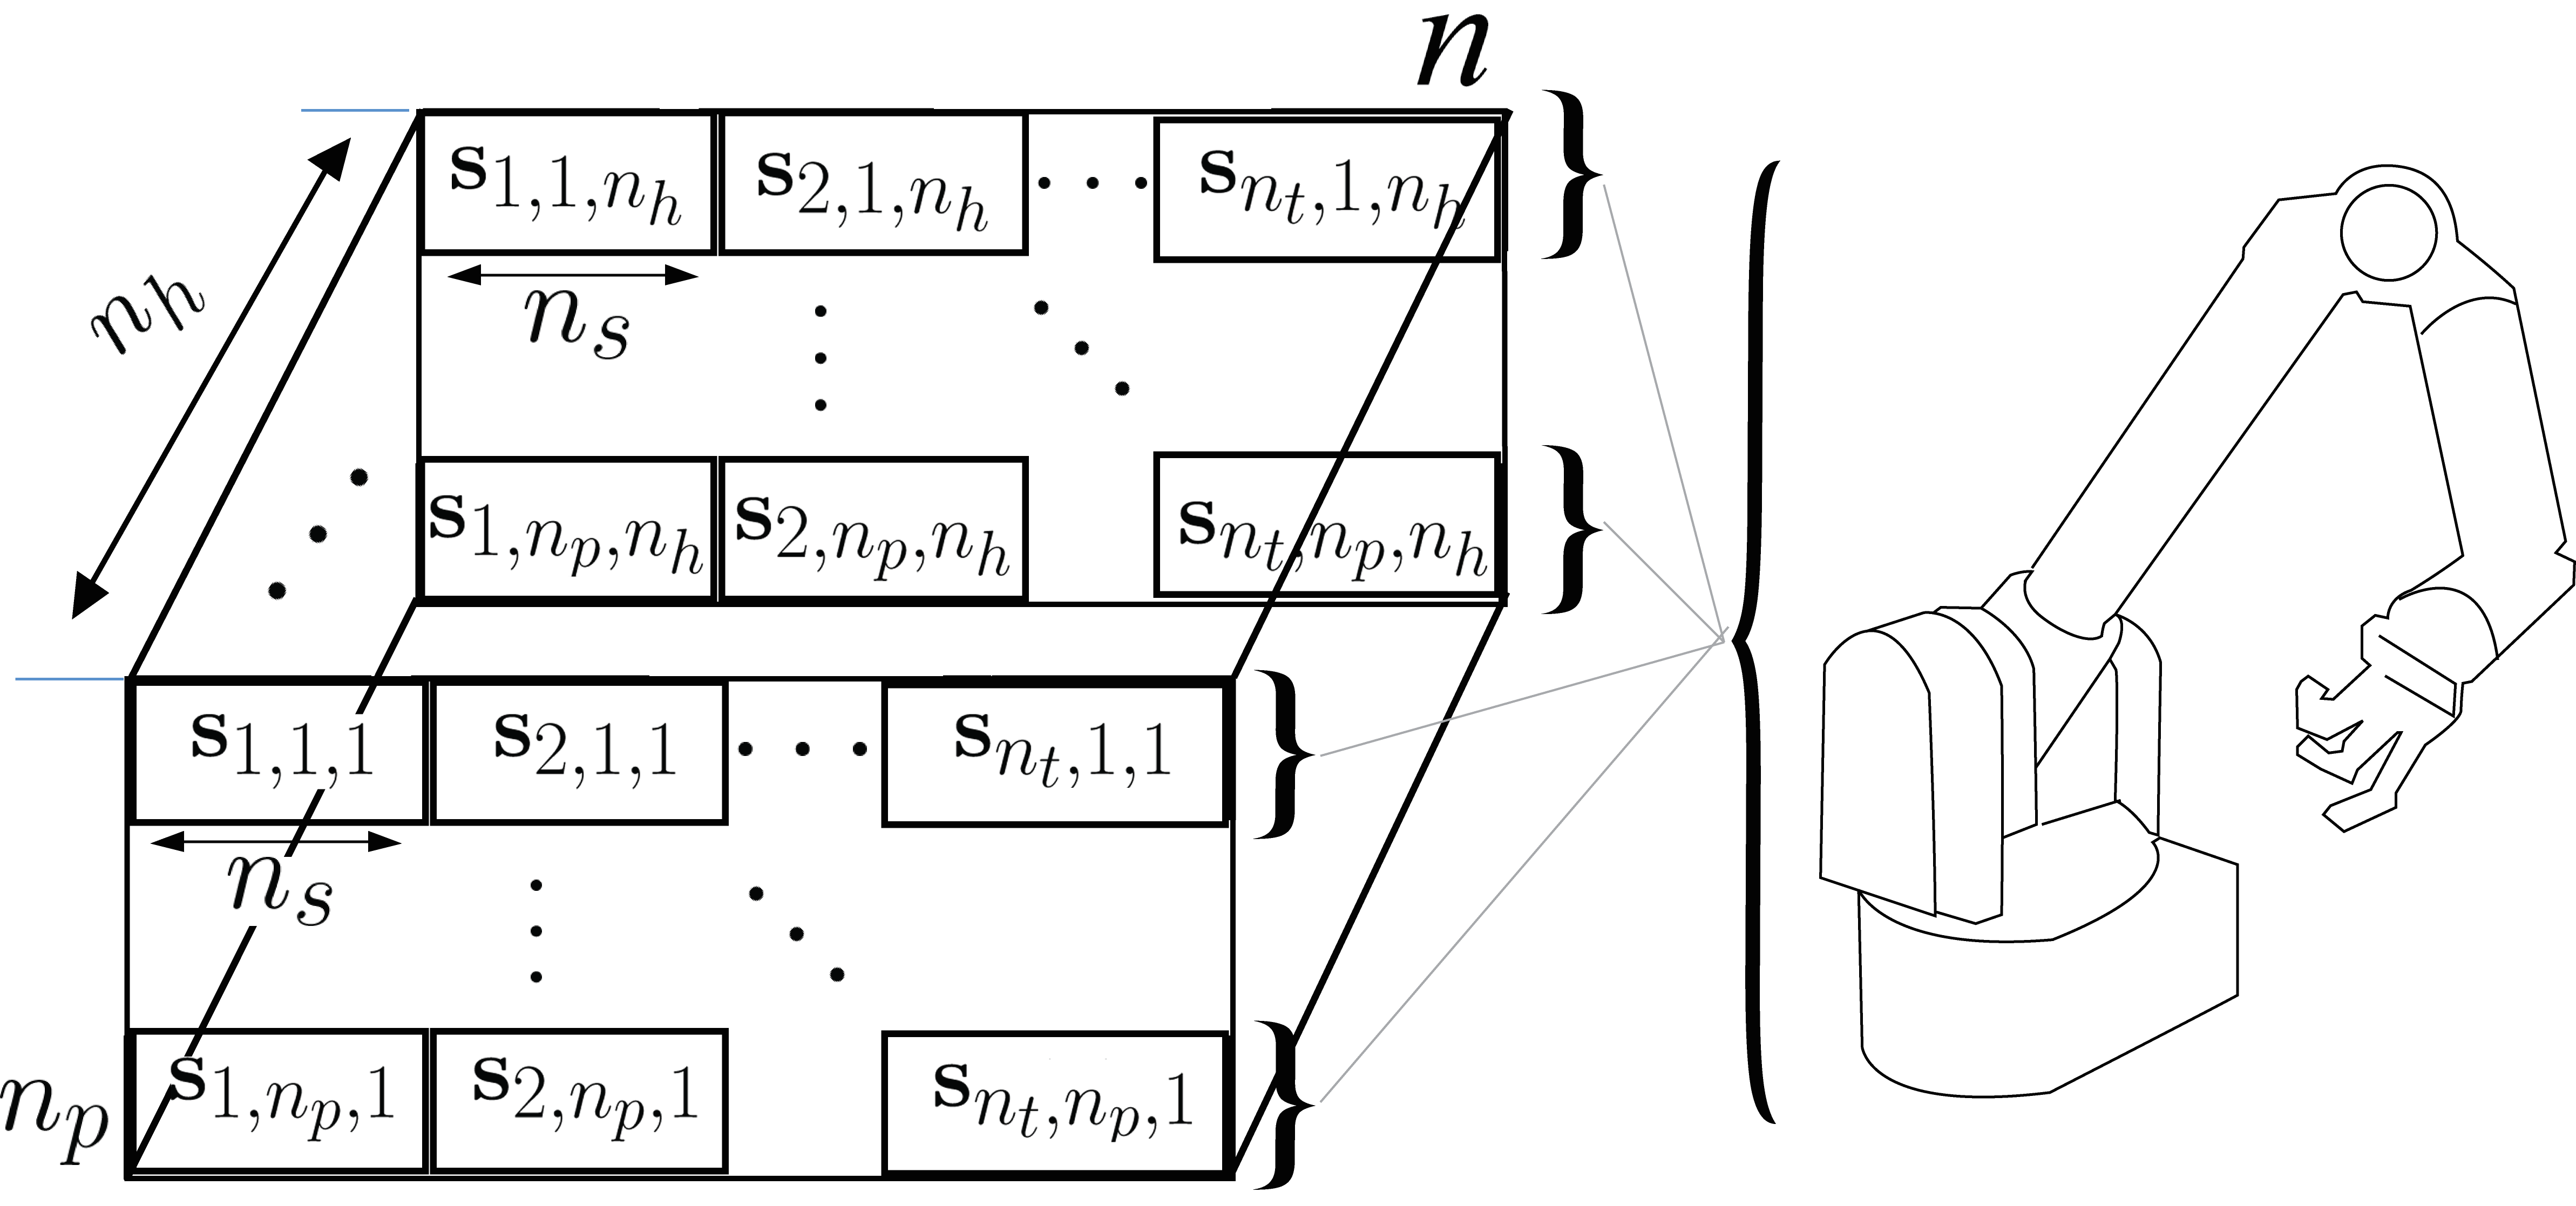
\includegraphics[width=\linewidth]{images/X_defn}  %% mass predictions
    \caption{$\mathbf{X}$}
    \label{fig:X_defn}
  \end{subfigure}
  %}
  %\fbox{
  ~~
  \begin{subfigure}[t]{0.43\linewidth}
    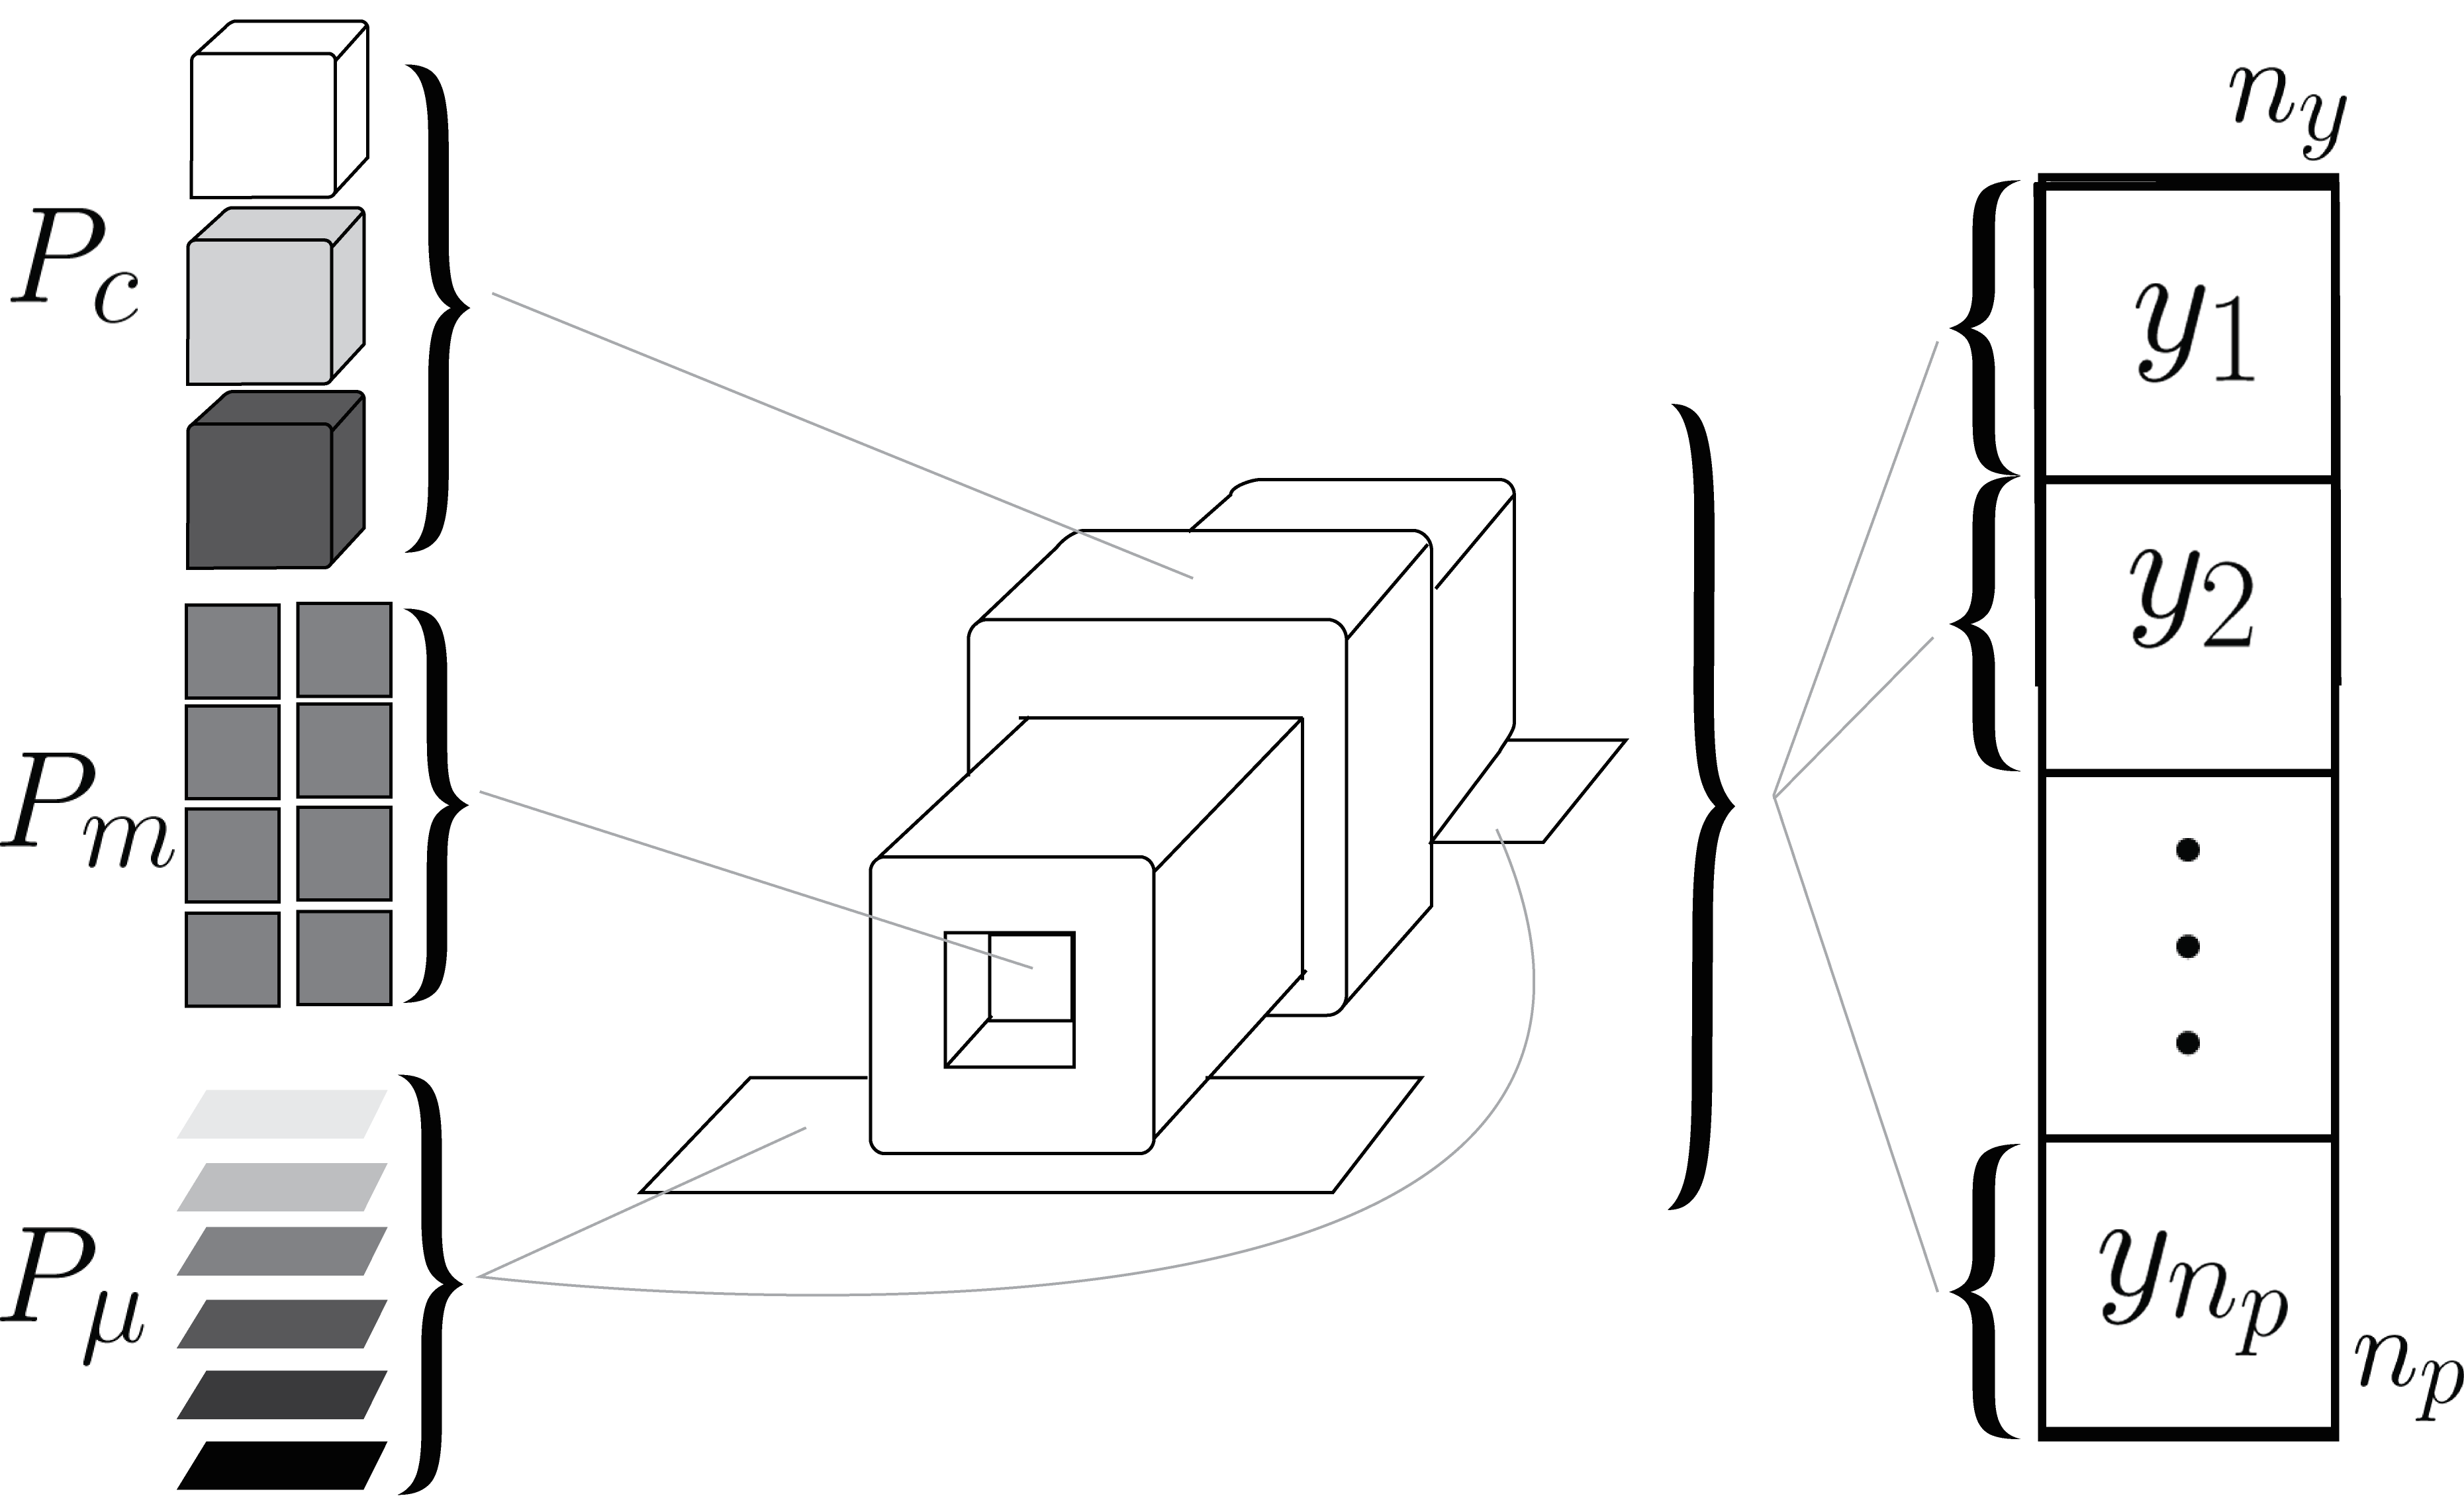
\includegraphics[width=\linewidth]{images/Y_defn}  %% mass predictions
    \caption{$\mathbf{Y}$}% provided}
    \label{fig:Y_defn}
  \end{subfigure}
  %}
  \caption{Collection of data matrix $\mathbf{D} = (\mathbf{X},\mathbf{Y})$: (a) data $\mathbf{X}$ are collected across all trials and environments; (b) environmental quantities $\mathbf{Y}$ are provided, which express each of $n_p = 144$ environments as $n_y=3$ floating point numbers.}
\end{figure}

%%% define the example motion and its purpose
The manipulation task considered is shown in Figure~\ref{fig:topple}. 
The end effector pushes down on a foam-encapsulated block, causing it to topple, then pushes the block back to its starting position against the wall.
A prescribed joint-space trajectory to achieve this manipulation task is provided by a human expert via kinesthetic teaching.
%TODO: is this really standard?
Upon replay, the robot tracks the given trajectory using standard computed-torque control.
We assume the trajectory is robust in two ways: (1) repeating the trajectory causes repeated rotations of the block, and (2) the same trajectory remains successful in toppling blocks for all mass, friction, and compliance values.
The use of a prescribed trajectory also implies an approximate correspondence between the current elapsed time within a motion and the manipulation phase.  
%While there is, by definition, no need for motion adaptation in this experimental setup, 
%The ability to predict environment properties such as mass, friction, and compliance in real-time is, we believe, an important prelude to enabling online motion adaptation.%adaptation of motions based on sensory data.

%%% define sensory data 
Each sensory sample collected at each timestep of the prescribed trajectory is defined by a sensory data stream:
\begin{equation}
\mathbf{s}\in\mathbb{R}^{n_s}:
(\rho,\dot{\rho},\tau,p,\omega,f,\alpha)
\end{equation}
  where $\rho,\dot{\rho},\tau\in\mathbb{R}^{7}$ represent respectively the angles, velocities and torque measurements of each of the seven joints of the manipulator arm, $p\in\mathbb{R}^{7}$ gives the end effector's pose measurements (3D position and 4D quaternion), $\omega \in\mathbb{R}^{6}$ is the task wrench measured via the force-torque sensor mounted to the wrist of the robot, $f \in\mathbb{R}^{4}$ are torque measurements for the joints in the robot hand, and $\alpha \in\mathbb{R}^{72}$ are tactile sensor measurements on each of the three fingers, reshaped into a single vector.

%The above definition of $s$ is valid when all sensors onboard the robot are used.
%We also perform experiments where the hand is replaced with a rigid spherical probe; thus changing both the kinematics of the arm and the sensory stream $s$ used to learn the predictive model and make subsequent predictions.

%We also build models where the robot hand is replaced by a spherical probe that is mounted to the force/torque sensor.
%For this scenario, a reduced version of $\mathbf{s}$ is defined by dropping the measurements associated with the robot hand.

A single execution of the manipulation task leads to the capture of a sensory stream, $\mathbf{x}\in\mathbb{R}^{n}$, which consists of the observations of $n_s$ sensor readings each sampled at $n_t$ points in time, and then stacked into a single vector; here, $n=n_s \times n_t$. 
%All the elements of $\mathbf{x}$ are standardized to have a zero mean and a variance of one, as measured across all trials and properties.
%This ensures that all the sensory measurements have approximately the same scale, irrespective of their origin.

%%% define environment properties 
The environment properties to be predicted from the sensory stream data are given by $\mathbf{y}\in\mathbb{R}^{3}: (m,\mu,c)$, where $m$ is the object mass, $\mu$ the coefficient of friction between the object and its support surface, and $c$ is the material compliance of the object.

%%% define training data 
In order to learn a predictive model $\mathbf{y}=f(\mathbf{x})$, training data is first gathered for $n_p$ different combinations of the environment properties, i.e., variations of mass, compliance, and friction.
For each setting, the task is repeated $n_h$ times in each environment.
The final dataset is thus defined by the following data pairs:
\begin{equation}   \mathbf{D} = (\mathbf{X},\mathbf{Y}) = \{ (\mathbf{x}_{p,h},\mathbf{y}_{p})~\lvert~p\in[1\cdots n_p],h\in[1\cdots n_h] \}. \end{equation} 


This dataset is used to learn the predictive model that we now describe.


%-------------------------------------------------------------------------------------------------------------------------------------------------
\section{Prediction Framework}

%%%%DMT%%%%
%TODO: recap on why feature selection is important (i.e. to reduce amount of data to be streamed from the robot to prediction system)
%DONE: develop an intuition for $\Gamma$ (look at Pais et al) - a figure demonstrating $\Gamma$ would help here
%TODO: form (cite?) theoretical basis for why $\Gamma$ works (Pais et al)
%TODO: propose a strategy for how this will carry over to different tasks
%TODO: can temporal information be leveraged at all (moving windows, wavelets)?
%TODO: take out classification and stick with regression throughout
%%%%%%%%%%%


%%% the predictive model

Given a new sensory stream, $\mathbf{x}_{new}$, which consists of $n_t$ samples of $\mathbf{s}$, we wish to predict the environment properties $\mathbf{y}$.
We develop a two-stage solution that consists of 
(i) selecting the most {\em relevant} input features from $\mathbf{x}$, and 
(ii) using partial least squares (PLS) to further learn a more compact latent linear subspace that is well suited to predicting environment properties.
%%%%%
%%DMT modified for simplicity 
%As we will show in the results, PLS property predictions without the initial feature selection step are not always sufficiently accurate.
%, despite its ability to exploit correlations between inputs and between inputs and outputs.
%%%%%
We now discuss these two stages in further detail.

\subsection{Feature Selection via the Task Variance Ratio}
\label{sec:feature_selection}

\begin{figure}[tb]
  \centering
  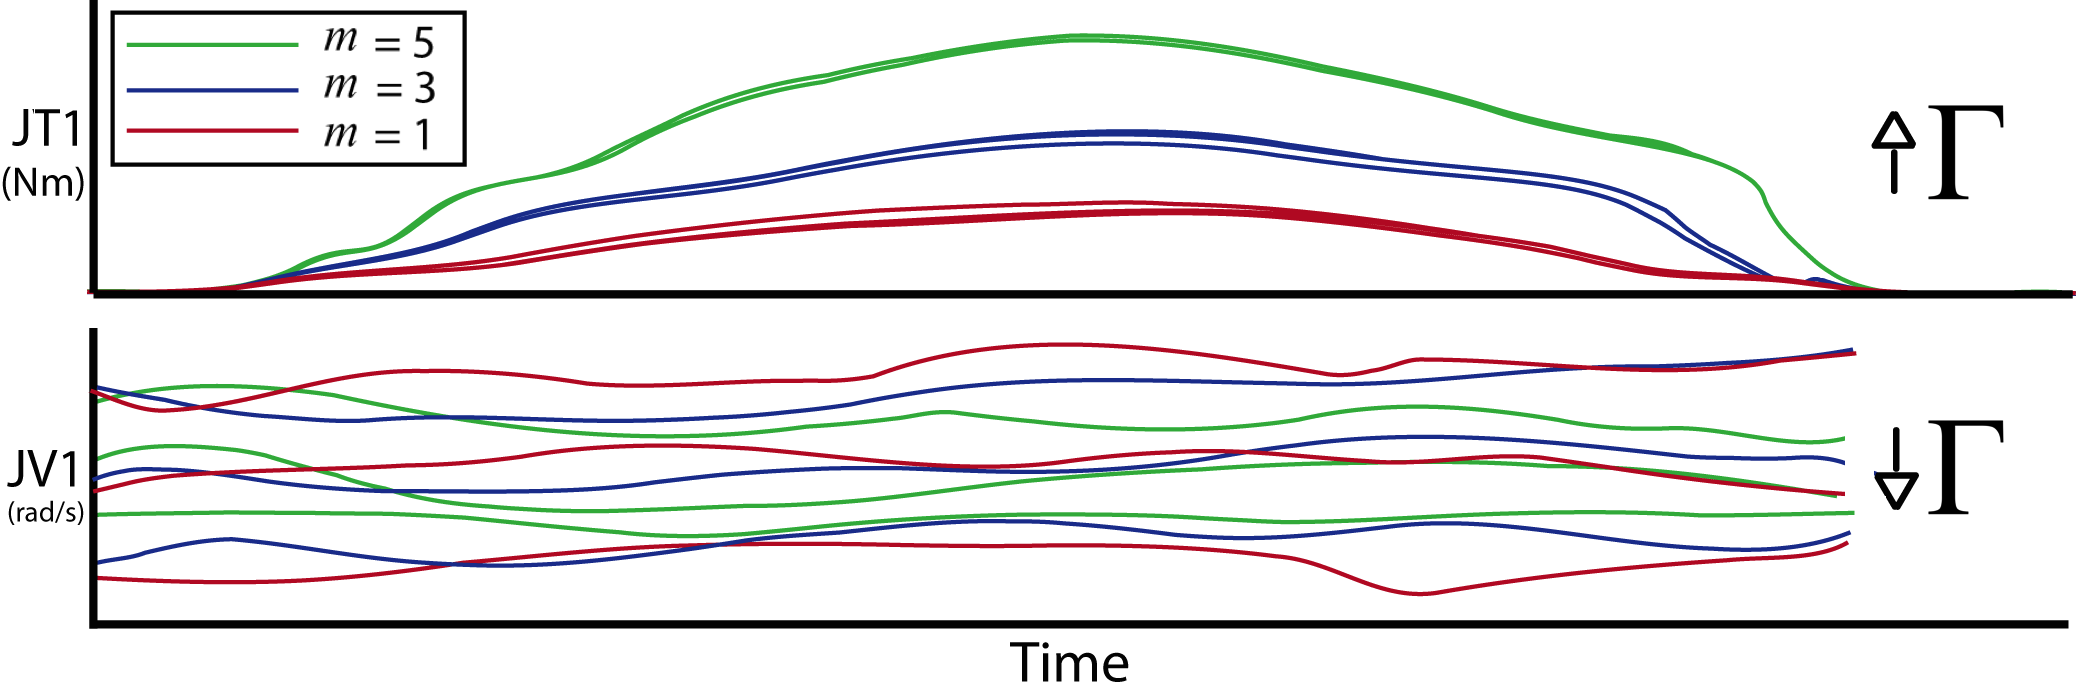
\includegraphics[width=\linewidth]{images/TVR_intuition}
  \caption{Intuition behind the task variance ratio ($\Gamma$) algorithm. We wish to select good sensors (at each time-phase) which exhibit low variance when the environment remains constant and high variance when the environment changes. Colors signify distinct environments. Multiple lines of the same color signify repeated trials within the same environment.}
  \label{fig:TVR_intuition}
\end{figure}

%\begin{figure}[t!]
%  %\fbox{
%  \begin{subfigure}[t]{0.5\linewidth}
%    \includegraphics[width=\linewidth]{images/mean_property}  %% mass predictions
%    \caption{$\mathbf{x}_{p}$}
%    \label{fig:mean_property}
%  \end{subfigure}
%  %}
%  %\fbox{
%  \begin{subfigure}[t]{0.46\linewidth}
%    \includegraphics[width=\linewidth]{images/mean_trial}  %% mass predictions
%    \caption{$\mathbf{x}_{h}$}
%    \label{fig:mean_trial}
%  \end{subfigure}
%  %}
%  %\fbox{
%  \\
%  \begin{subfigure}[t]{0.46\linewidth}
%    \includegraphics[width=\linewidth]{images/var_property}  %% mass predictions
%    \caption{$\sigma^2_{enviro}$}% provided}
%    \label{fig:var_property}
%  \end{subfigure}
%  %}
%  \begin{subfigure}[t]{0.5\linewidth}
%    \includegraphics[width=\linewidth]{images/var_trial}  %% mass predictions
%    \caption{$\sigma^2_{trial}$}% provided}
%    \label{fig:var_trial}
%  \end{subfigure}
%  \caption{Visualization of $\Gamma$ calculation. First, mean sensor readings across property sets (a) and trials (b) are calculated from data $\mathbf{X}$. Next, the variance of these mean sensor readings are calculated (c,d). Finally $\Gamma$ is defined as the ratio of the two variance vectors.}
%%a) mean sensor readings within each property set and across all trials; b) mean sensor readings within each trial and across all property sets; c) variance of mean sensor readings across property sets; d) variance of mean sensor readings across trials.}
%  \label{fig:TVR_calculation}
%\end{figure}

%%%%%
%%DMT added:
%As mentioned previously, due to limited resources, systems embedded on robotic hardware typically cannot process large amounts of input data in real-time.
%%%%%%
%To cope with the high dimensional nature of the sensory stream data, we first describe a selection mechanism that is well suited to identifying specific sensors and sample times that are likely to be informative for the prediction problem.
%\begin{equation}   \mathbf{D} = (\mathbf{X},\mathbf{Y}) = \{ (\mathbf{x}_{p,h},\mathbf{y}_{p})~\lvert~p\in[1\cdots n_p],h\in[1\cdots n_h] \}. \end{equation} 
We define the {\em Task Variance Ratio ($\Gamma$)} vector as
%   \begin{equation}  \Gamma = {\frac{\sigma^2_{enviro}}{\sigma^2_{trial}} | } ,\end{equation}
\begin{equation} \Gamma = \{\Gamma^i=\frac{\mathit{Var}_i^{enviro}}{\mathit{Var}_i^{trial}}~\lvert~i\in[1\cdots n] \} \end{equation}
where $\mathit{Var}_i^{trial}$ models the variance of a given element of $\mathbf{X}$ across all trials, 
and $\mathit{Var}_i^{enviro}$ models the variance of the same element across all environments. 
Specifically, 
   %\begin{equation}\sigma^2_{trial} = \frac{\sum{(\mathbf{x}_{h}-\bar{\mathbf{x}_{h}})^2}}{n_h-1},\end{equation}
  \begin{equation}\mathit{Var}_i^{trial}=\frac{\sum_{h=1}^{n_h}({\mathit{x}_{i,h})^2}-\frac{(\sum_{h=1}^{n_h}{\mathit{x}_{i,h}})^2}{n_h}}{n_h-1}\end{equation}
%i.e., the variance of the given element as computed using all available measurements (all properties $p$ and trials $h$) in $\mathbf{D}$, 
and 
   %\begin{equation}\sigma^2_{enviro} = \frac{\sum{(\mathbf{x}_{p}-\bar{\mathbf{x}_{p}})^2}}{n_p-1},\end{equation}
  \begin{equation}\mathit{Var}_i^{enviro} = \frac{\sum_{p=1}^{n_p}{(\mathit{x}_{i,p})^2}-\frac{(\sum_{p=1}^{n_p}{\mathit{x}_{i,p}})^2}{n_p}}{n_p-1}\end{equation}
%i.e., the mean of the $n_p$ variances that can be computed when measurements are grouped according to environment properties.
for all $i \in [1\cdots n]$.

A large value of $\Gamma_i$ indicates a good feature, as it implies that variation occurs as changes to the environment take effect, while observable noise between repeated trials in the same environment is relatively small.

%\begin{equation}\mathbf{X}_{h} = \frac{1}{n_p}\sum_{p=1}^{n_p}{\mathbf{x}_{p,h}}~\lvert~ h\in[1\cdots n_h]\end{equation} and

The feature selection is then implemented using a simple threshold function to produce a reduced input matrix $\mathbf{X}^*$:
   \begin{equation} \mathbf{X}^* = \mathbf{X}_p \cdot diag(\Gamma > \Gamma_{\min}),\end{equation} 
where
\begin{equation}\mathbf{X}_{p} = \frac{1}{n_h}\sum_{h=1}^{n_h}{\mathbf{x}_{p,h}}~\lvert~ p\in[1\cdots n_p],\end{equation} 
$diag(v)$ produces a square matrix with the elements of $v$ across the diagonal, and $\Gamma_{min}$ is chosen such that the desired number of elements of $\Gamma$ are selected.
%where $i\in[1\cdots n_sn_t]$, $p\in[1\cdots n_p]$, and $h\in[1\cdots n_h]$.
%\begin{equation} 
%\mathbf{x}_i^*= 
%\left\{
%\begin{matrix*}[l]
%1\; if\;  \Gamma_i >\Gamma_{min}
%\\ 
%0\;\; otherwise
%\end{matrix*}
%\right.
%\end{equation}
The resulting reduced dataset is given by
\begin{equation}   \mathbf{D}^* = (\mathbf{X}^*,\mathbf{\mathbf{Y}}) = \{ (\mathbf{x^*}_{p},\mathbf{y}_{p})~\lvert~ p\in[1\cdots n_p] \}. \end{equation} 

In this way, we identify features in $\mathbf{X}$ that exhibit small variation across repeated trials when the environment is kept constant and exhibit large variations as the environment changes (see Figure~\ref{fig:TVR_intuition}), which we approximate as the degree of relevance of the sensor reading to predicting environment properties.

\subsection{Property prediction with Partial Least Squares}
\label{sec:PLS}

% is an effective prediction method in high-dimensional settings such as the one encountered here.

The PLS algorithm provides us with an estimated weighting matrix $\mathbf{\beta} \in \mathbb{R}^{c\times n_y}$, where $c$ is a parameter denoting the number components to factor.

$\beta$ is calculated iteratively according to the following algorithm:
first, define 
\begin{equation}
\begin{aligned}
A_0& = \mathbf{X^{*T}}\mathbf{Y}, \\
M_0& = \mathbf{X^{*T}}\mathbf{X^*},&& \text{and} \\
C_0& = I,\\
\end{aligned}
\end{equation}
then iterate
\begin{equation}
\begin{aligned}
q_j& = eigv1(A^T_{j-1}A_{j-1}) && \text{$q_j \rightarrow$ dominant eigenvector} \\
w_j& = A_{j-1}q_j \\%&& \text{blah}\\
c_j& = w^T_jM_{j-1}w_j \\%&& \text{blah}\\
w_j& = \frac{w_j}{\sqrt{c_j}} && \text{store into column j of W}\\
r_j& =M_{j-1}w_j && \text{store into column j of R}\\
q_j& =A^T_{j-1}w_j && \text{store into column j of Q}\\
v_j& =\eta C_jp_j && \text{$\eta \rightarrow$ normalizing constant}\\
C_j& =C_{j-1}-v_jv_j^T \\%&& \text{blah}\\
A_j& =C_jA_{j-1} \\%&& \text{blah} 
\end{aligned}
\end{equation}
for all $j \in [1 \cdots c]$.
With $R$, $Q$ and $W$ assembled, we now compute: 

\begin{equation}
%\begin{aligned}
\beta = WQ^T
%\end{aligned}
\end{equation}

  %\begin{equation} \beta = PLS(\mathbf{D}^*). \end{equation}
Finally, we use $\beta$ at runtime to predict environment properties:
  \begin{equation} \mathbf{\hat{y}} = \mathbf{\beta} \cdot \mathbf{x^*_{new}} \end{equation}

Data from multiple haptic sensors are likely to be highly correlated, e.g. Cartesian force experienced by the hand and tactile pressure readings at the fingertips.
In addition, there is likely to be significant correlation between sensor readings over time.
Lastly, there are correlations between the input dimensions and output dimensions.
The existance of these correlations are ideal in the application of the PLS  regression method \cite{Tobias1995}.
%--------------------------------------------------------------------------------------------------------------
